\documentclass[journal,12pt,twocolumn]{IEEEtran}
%
\usepackage{setspace}
\usepackage{gensymb}
%\doublespacing
\singlespacing

\usepackage[cmex10]{amsmath}
\usepackage{amsthm}
%\usepackage{iithtlc}
\usepackage{mathrsfs}
\usepackage{txfonts}
\usepackage{stfloats}
\usepackage{bm}
\usepackage{cite}
\usepackage{cases}
\usepackage{subfig}
%\usepackage{xtab}
\usepackage{longtable}
\usepackage{multirow}

\usepackage{enumitem}
\usepackage{mathtools}
\usepackage{steinmetz}
\usepackage{tikz}
\usepackage{circuitikz}
\usepackage{verbatim}
\usepackage{tfrupee}
\usepackage[breaklinks=true]{hyperref}
\usepackage{tkz-euclide} % loads  TikZ and tkz-base
\usetikzlibrary{calc,math}
\usepackage{listings}
    \usepackage{color}                                            %%
    \usepackage{array}                                            %%
    \usepackage{longtable}                                        %%
    \usepackage{calc}                                             %%
    \usepackage{multirow}                                         %%
    \usepackage{hhline}                                           %%
    \usepackage{ifthen}                                           %%
  %optionally (for landscape tables embedded in another document): %%
    \usepackage{lscape}     
\usepackage{multicol}
\usepackage{chngcntr}
%\usepackage{enumerate}

%\usepackage{wasysym}
%\newcounter{MYtempeqncnt}
\DeclareMathOperator*{\Res}{Res}
%\renewcommand{\baselinestretch}2
\renewcommand\thesection{\arabic{section}}
\renewcommand\thesubsection{\thesection.\arabic{subsection}}
\renewcommand\thesubsubsection{\thesubsection.\arabic{subsubsection}}

\renewcommand\thesectiondis{\arabic{section}}
\renewcommand\thesubsectiondis{\thesectiondis.\arabic{subsection}}
\renewcommand\thesubsubsectiondis{\thesubsectiondis.\arabic{subsubsection}}

% correct bad hyphenation here
\hyphenation{op-tical net-works semi-conduc-tor}
\def\inputGnumericTable{}                                 %%

\lstset{
%language=C,
frame=single, 
breaklines=true,
columns=fullflexible
}
%\lstset{
%language=tex,
%frame=single, 
%breaklines=true
%}

\begin{document}
%


\newtheorem{theorem}{Theorem}[section]
\newtheorem{problem}{Problem}
\newtheorem{proposition}{Proposition}[section]
\newtheorem{lemma}{Lemma}[section]
\newtheorem{corollary}[theorem]{Corollary}
\newtheorem{example}{Example}[section]
\newtheorem{definition}[problem]{Definition}
\newcommand{\BEQA}{\begin{eqnarray}}
\newcommand{\EEQA}{\end{eqnarray}}
\newcommand{\define}{\stackrel{\triangle}{=}}
\bibliographystyle{IEEEtran}
\providecommand{\mbf}{\mathbf}
\providecommand{\pr}[1]{\ensuremath{\Pr\left(#1\right)}}
\providecommand{\qfunc}[1]{\ensuremath{Q\left(#1\right)}}
\providecommand{\sbrak}[1]{\ensuremath{{}\left[#1\right]}}
\providecommand{\lsbrak}[1]{\ensuremath{{}\left[#1\right.}}
\providecommand{\rsbrak}[1]{\ensuremath{{}\left.#1\right]}}
\providecommand{\brak}[1]{\ensuremath{\left(#1\right)}}
\providecommand{\lbrak}[1]{\ensuremath{\left(#1\right.}}
\providecommand{\rbrak}[1]{\ensuremath{\left.#1\right)}}
\providecommand{\cbrak}[1]{\ensuremath{\left\{#1\right\}}}
\providecommand{\lcbrak}[1]{\ensuremath{\left\{#1\right.}}
\providecommand{\rcbrak}[1]{\ensuremath{\left.#1\right\}}}
\theoremstyle{remark}
\newtheorem{rem}{Remark}
\newcommand{\sgn}{\mathop{\mathrm{sgn}}}
\providecommand{\abs}[1]{\left\vert#1\right\vert}
\providecommand{\res}[1]{\Res\displaylimits_{#1}} 
\providecommand{\norm}[1]{\left\lVert#1\right\rVert}
\providecommand{\norm}[1]{\lVert#1\rVert}
\providecommand{\mtx}[1]{\mathbf{#1}}
\providecommand{\mean}[1]{E\left[ #1 \right]}
\providecommand{\fourier}{\overset{\mathcal{F}}{ \rightleftharpoons}}
%\providecommand{\hilbert}{\overset{\mathcal{H}}{ \rightleftharpoons}}
\providecommand{\system}{\overset{\mathcal{H}}{ \longleftrightarrow}}
	%\newcommand{\solution}[2]{\textbf{Solution:}{#1}}
\newcommand{\solution}{\noindent \textbf{Solution: }}
\newcommand{\cosec}{\,\text{cosec}\,}
\providecommand{\dec}[2]{\ensuremath{\overset{#1}{\underset{#2}{\gtrless}}}}
\newcommand{\myvec}[1]{\ensuremath{\begin{pmatrix}#1\end{pmatrix}}}
\newcommand{\mydet}[1]{\ensuremath{\begin{vmatrix}#1\end{vmatrix}}}
%\numberwithin{equation}{section}
\numberwithin{equation}{subsection}
\makeatletter
\@addtoreset{figure}{problem}
\makeatother
\let\StandardTheFigure\thefigure
\let\vec\mathbf
%\renewcommand{\thefigure}{\theproblem.\arabic{figure}}
\renewcommand{\thefigure}{\theproblem}
%\setlist[enumerate,1]{before=\renewcommand\theequation{\theenumi.\arabic{equation}}
%\counterwithin{equation}{enumi}
%\renewcommand{\theequation}{\arabic{subsection}.\arabic{equation}}
\def\putbox#1#2#3{\makebox[0in][l]{\makebox[#1][l]{}\raisebox{\baselineskip}[0in][0in]{\raisebox{#2}[0in][0in]{#3}}}}
     \def\rightbox#1{\makebox[0in][r]{#1}}
     \def\centbox#1{\makebox[0in]{#1}}
     \def\topbox#1{\raisebox{-\baselineskip}[0in][0in]{#1}}
     \def\midbox#1{\raisebox{-0.5\baselineskip}[0in][0in]{#1}}
\vspace{3cm}
\title{Assignment 1}
\author{P VENKATA PRANEETH}
\maketitle
\newpage
%\tableofcontents
\bigskip
\renewcommand{\thefigure}{\theenumi}
\renewcommand{\thetable}{\theenumi}
Find Python Codes from below link 
%
\begin{lstlisting}
https://github.com/praneeth2720/Assignment-1/blob/main/vectors.py
\end{lstlisting}
%
and latex codes from 
%
\begin{lstlisting}
https://github.com/praneeth2720/Assignment-1
\end{lstlisting}
%
\section{CBSE 10th 2008 paper.}
% \subsection{Question 1}
\subsection{Question 22}
% \renewcommand{\theequation}{\theenumi}
\item 
\numberwithin{equation}
 The mid-points of the side of triangle are (3,4) ,(4,6) and (5,7). Find the coordinates of the vertices of the triangle.
\subsection{Solution}
Let the mid pints of the sides of triangle are \\
\vec{P}=\myvec{3 \\ 4} \
\vec{Q}=\myvec{4 \\ 6} \
\vec{R}=\myvec{5 \\ 7} \\
\ Let assume coordintes of the vertices of triangle as \\
\vec{A}\
\vec{B}\
\vec{C}\
\begin{center}
By using section formula \\
\end{center}
\begin{align}
\frac{\vec{A}+ \vec{B}}{2} &= $\vec{P}$ \\
\frac{\vec{B} + \vec{C}}{2} &= $\vec{Q}$\\
\frac{\vec{A} + \vec{C}}{2} &= $\vec{R}$\\
\end{align}
\begin{align}
\vec{A+B} &= $2\vec{P}$\\
\vec{B+C} &= $2\vec{Q}$\\
\vec{A+C} &= $2\vec{R}$\\
\end{align}

\\ Let us consider the above three equations as \  
\\ And \myvec{$\vec{I} & $\vec{I} & 0 \\ 0 & $\vec{I} & $\vec{I} \\ $\vec{I} & 0 & $\vec{I} \\ } as \vec{T} 

\begin{align}
\myvec{\vec{I} & \vec{I} & 0 \\ 0 & \vec{I} & \vec{I} \\ \vec{I} & 0 & \vec{I} \\ }\myvec{\vec{A}  \\ \vec{B} \\ \vec{C} \\ } &= 2 \myvec{\vec{P}\\ \vec{Q} \\ \vec{R}} 
\end{align}
\\now multiplying each side with \vec{T}^{-1} 
\ we get\\
\begin{center}
 \myvec{\vec{A}  \\ \vec{B} \\ \vec{C} \\ } &= 2 $\frac{1}{2}\ $\myvec{1 & 1 & -1 \\ -1 & 1 & 1 \\ 1 & -1 & 1 \\ } \myvec{\vec{P}  \\ \vec{Q} \\ \vec{R}}  
\end{center}
\begin{align}
\myvec{\vec{A}  \\ \vec{B} \\ \vec{C} \\ } &= \myvec{\vec{P} + \vec{Q}  -\vec{R}\\ \vec{-P} +\vec{Q} + \vec{R} \\ \vec{P}  -\vec{Q} + \vec{R} \\ }\\
\myvec{\vec{A}  \\ \vec{B} \\ \vec{C} \\ } &= \myvec{ $\myvec{4 \\ 5} \\ $\myvec{2 \\ 3} \\ $\myvec{6 \\ 9} }    
\end{align}
 \therefore $by comparing rows of each side we get the vertices of triangle.They are as follows \\
\vec{A}=\myvec{4 \\ 5} \
\vec{B}=\myvec{2 \\ 3} \
\vec{C}=\myvec{6 \\ 9} \\
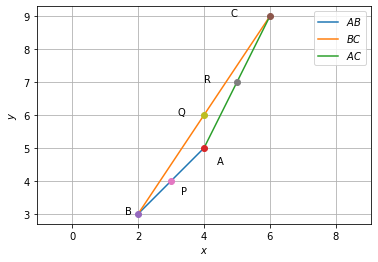
\includegraphics[width=\columnwidth]{VEC.png}
\caption{}
\label{fig:straight lines}	
\end{figure}

\end{document}
